\begin{center}
{\Huge Química}

{\Large Formulario}
\end{center}
\tableofcontents
\newpage

\begin {multicols}{2}

\hypertarget{conversiones}{%
\section{Conversiones}\label{conversiones}}

\hypertarget{peso}{%
\subsubsection{Peso}\label{peso}}

\(\text{1 lb}=\text{453,6 g}\)

\(\text{1 kg}=\text{2,2 lb}\)

\(\text{1 oz}=\text{28,35 g}\)

\hypertarget{longitud}{%
\subsubsection{Longitud}\label{longitud}}

\(\text{1 mi}=\text{1,61 km}\)

\(\text{1 m}=\text{3,28 ft}\)

\(\text{1 m}=39,4^{"}\)

\(1^{"}=\text{2,54 cm}\)

\hypertarget{gases}{%
\subsubsection{Gases}\label{gases}}

\(\text{1 atm}=\text{760 mmHg}\)

\(\text{1 atm}=\text{101,3 kPa}\)

\(\text{1 atm}=\text{14,696 psi}\)

\(\text{1 torr}=\text{1 mmHg}\)

\(\text{1 torr}=\text{133,32 Pa}\)

\(\text{1 bar}=10^{5}\text{ Pa}\)

\hypertarget{termodinuxe1mica}{%
\subsubsection{Termodinámica}\label{termodinuxe1mica}}

\(\text{1 cal}=\text{4,18 J}\)

\(\text{1 atmL}=\text{101,3 J}\)

\hypertarget{propiedades-intensivas}{%
\section{Propiedades intensivas}\label{propiedades-intensivas}}

\(m=dv\)

\begin{quote}
(s), (l) = g/cm³; (g) = g/m³
\end{quote}

\(\textcelsius=(F-32)\frac{5}{9}\)

\(F=\frac{9}{5}\textcelsius+32\)

\(K=\textcelsius+273,15\)

\hypertarget{estequiometruxeda}{%
\section{Estequiometría}\label{estequiometruxeda}}

\hypertarget{unidades-de-cantidad}{%
\subsubsection{Unidades de cantidad}\label{unidades-de-cantidad}}

\(1uma=\frac{g}{mol}\)

\begin{quote}
El peso atómico se mide en uma's.
\end{quote}

\(1g=6,022{\cdot}10^{23}uma\)

\(N_{A}/L=6,022{\cdot}10^{23}\text{partículas}\)

\hypertarget{isuxf3topo}{%
\subsubsection{Isótopo}\label{isuxf3topo}}

\(\bar{m}=m_{1}Ab_{1}+...+m_{n}Ab_{n}\)

\hypertarget{composiciuxf3n-porcentual}{%
\subsubsection{Composición porcentual}\label{composiciuxf3n-porcentual}}

\(Mr={\Sigma}Ar\)

\(\%X=\frac{nAr}{Mr}100\%\)

\hypertarget{fuxf3rmulas-quuxedmicas}{%
\subsubsection{Fórmulas químicas}\label{fuxf3rmulas-quuxedmicas}}

\(FM=nFE\)

\(m=nMr\)

\hypertarget{reacciones}{%
\section{Reacciones}\label{reacciones}}

\hypertarget{rendimiento}{%
\subsubsection{Rendimiento}\label{rendimiento}}

\(\%r=\frac{\text{real}}{\text{teórico}}100\%\)

\hypertarget{soluciones}{%
\section{Soluciones}\label{soluciones}}

\(C_1V_1=C_2V_2\)

\(m_{\text{solución}}=m_{soluto}+m_{solvente}\)

\(V_{\text{solución}}=V_{soluto}+V_{solvente}\)

\hypertarget{molaridad-m}{%
\subsubsection{\texorpdfstring{Molaridad
\((M)\)}{Molaridad (M)}}\label{molaridad-m}}

\(M=\frac{n_{soluto}}{{\langle}1{\rangle}{dm^3}_{\text{solución}}}\)

\hypertarget{molalidad-eta}{%
\subsubsection{\texorpdfstring{Molalidad
\((\eta)\)}{Molalidad (\textbackslash eta)}}\label{molalidad-eta}}

\(\eta=\frac{n_{soluto}}{{\langle}1{\rangle}kg_{solvente}}\)

\hypertarget{fracciuxf3n-molar-x}{%
\subsubsection{\texorpdfstring{Fracción molar
\((X)\)}{Fracción molar (X)}}\label{fracciuxf3n-molar-x}}

\(X_{A}=\frac{n_{A}}{{\langle}1{\rangle}n_{\text{solución}}}\)

\(X_{B}=\frac{n_{B}}{{\langle}1{\rangle}n_{\text{solución}}}\)

\(X_{A}+X_{B}=1\)

\hypertarget{porcentaje-en-masa-m_}{%
\subsubsection{\texorpdfstring{Porcentaje en masa
\((m_\%)\)}{Porcentaje en masa (m\_\textbackslash\%)}}\label{porcentaje-en-masa-m_}}

\(m_\%=\frac{g_{soluto}}{{\langle}100{\rangle}g_{\text{solución}}}{\cdot}100\%\)

\hypertarget{porcentaje-en-volumen-v_}{%
\subsubsection{\texorpdfstring{Porcentaje en volumen
\((V_\%)\)}{Porcentaje en volumen (V\_\textbackslash\%)}}\label{porcentaje-en-volumen-v_}}

\(V_\%=\frac{V_{soluto}}{V_{\text{solución}}}{\cdot}100\%\)

\hypertarget{partes-por-milluxf3n-ppm}{%
\subsubsection{\texorpdfstring{Partes por millón
\((ppm)\)}{Partes por millón (ppm)}}\label{partes-por-milluxf3n-ppm}}

\(m_\%=\frac{m_{soluto}}{m_{\text{solución}}}{\cdot}10^6\)

\hypertarget{gases-1}{%
\section{Gases}\label{gases-1}}

\(R=8,314\frac{J}{K{\cdot}mol}\)
\(R=0,0821\frac{atm{\cdot}L}{K{\cdot}mol}\)

\begin{quote}
Condiciones normales (CNTP): 1 atm, 0ºC

Condiciones estándar (TPE): 1 atm, 25ºC (temperatura ambiente)
\end{quote}

\hypertarget{ley-de-los-gases-ideales}{%
\subsubsection{Ley de los gases
ideales}\label{ley-de-los-gases-ideales}}

\(PV=nRT\)

\hypertarget{ecuaciuxf3n-de-estado}{%
\subsubsection{Ecuación de estado}\label{ecuaciuxf3n-de-estado}}

\(\frac{P_{1}V_{1}}{n_{1}T_{1}}=\frac{P_{2}V_{2}}{n_{2}T_{2}}\)

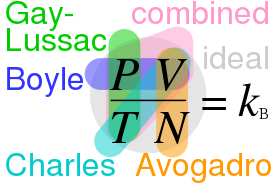
\includegraphics[width=0.2\textwidth,height=\textheight]{./media/ideal-gas-law-relationships.png}

\hypertarget{densidad-de-un-gas}{%
\subsubsection{Densidad de un gas}\label{densidad-de-un-gas}}

\(\rho=\frac{MrP}{RT}\)

\hypertarget{ley-de-dalton}{%
\subsubsection{Ley de Dalton}\label{ley-de-dalton}}

\(P_{A}=X_{A}P_{T}\)

\(P_{A}=\frac{n_{A}RT}{V}\)

\hypertarget{volumen-molar-de-un-gas}{%
\subsubsection{Volumen molar de un gas}\label{volumen-molar-de-un-gas}}

\(1mol=22,7dm^{3}\)

\begin{quote}
Posible a CNTP.
\end{quote}

\hypertarget{termodinuxe1mica-1}{%
\section{Termodinámica}\label{termodinuxe1mica-1}}

\hypertarget{trabajo-y-energuxeda}{%
\subsubsection{Trabajo y energía}\label{trabajo-y-energuxeda}}

\(W=-P{\Delta}V\Leftrightarrow W=-{\Delta}nRT\)

\({\Delta}U=Q+W\)

\begin{quote}
\(\begin{matrix}\text{\small{recibe}} & + \\ \text{\small{libera}} & -\end{matrix}\)
\end{quote}

\hypertarget{entalpuxeda}{%
\subsubsection{Entalpía}\label{entalpuxeda}}

\({\Delta}H=H_{productos}-H_{reactivos}\)

\textbf{Entalpía estándar de reacción}

\({\Delta}H_{\text{rxn}}^\circ=[c{\Delta}H_{f}^\circ(C)+d{\Delta}H_{f}^\circ(D)]-[a{\Delta}H_{f}^\circ(A)+b{\Delta}H_{f}^\circ(B)]\)

\textbf{Entalpía de una solución}

\({\Delta}H_{\text{soln}}=H_{\text{solución}}-H_{\text{componentes}}\)

\begin{quote}
\({\Delta}H>{\Delta}E→\text{compresión}\)

\({\Delta}H<{\Delta}E→\text{expansión}\)

\({\Delta}H={\Delta}E→\text{rxn que no produce cambio en moles}\)

\({\Delta}H_{\text{soln}}=0→\text{solución ideal}\)
\end{quote}

\hypertarget{calor}{%
\subsubsection{Calor}\label{calor}}

\(-Q_1=Q_2\)

\(Q=mc{\Delta}T\)

\(C=mc\)

\(c_{H_{2}O}=4,184\frac{J}{g\textcelsius}\)

\hypertarget{cuxe1lculos-de-un-sistema}{%
\subsubsection{Cálculos de un sistema}\label{cuxe1lculos-de-un-sistema}}

\(Q_{sis}={\Sigma}Q_{\text{Componentes}}\)

\textbf{Componentes}

\(Q_{sis}=0\Leftrightarrow\text{ningún calor entra o sale}\)

\(Q_{H_{2}O}=mc{\Delta}T\)

\(Q_{\text{aparato}}=C_{\text{aparato}}{\Delta}T\)

Reacción a P constante

\(Q_{\text{rxn}}={\Delta}H\)

Reacción a V constante

\(Q_{\text{rxn}}={\Delta}U\)

\hypertarget{cambio-de-fases}{%
\subsubsection{Cambio de fases}\label{cambio-de-fases}}

\({\Delta}H_{sub}={\Delta}H_{fus}+{\Delta}H_{vap}\)

\hypertarget{propiedades-coligativas}{%
\subsubsection{Propiedades coligativas}\label{propiedades-coligativas}}

\begin{quote}
\(^\circ=\text{puro}\)

\(_1=\text{solvente}\)

\(_2=\text{soluto}\)
\end{quote}

\(\text{Factor de Van't Hoff }(i)=\frac{\text{\# partículas productos}}{\text{\# partículas reactivos}}\)

\begin{quote}
Para no electrolitos es igual a uno.
\end{quote}

\textbf{Disminución de presión de vapor}

\(P_1=X_1P_1^\circ\)

\({\Delta}P=X_2P_1^\circ\)

\({\Delta}P=P_1^\circ-P_1\)

\textbf{Elevación del punto de ebullición}

\({\Delta}T_b=ik_{b_1}\eta\)

\({\Delta}T_b=T_{b_2}-T_{b_1}^\circ\)

\(T_b>T_b^\circ→{\Delta}T_b>0\)

\textbf{Disminución del punto de ebullición}

\({\Delta}T_f=ik_{f_1}\eta\)

\({\Delta}T_f=T_{f_2}^\circ-T_{f_1}\)

\(T_f^\circ>T_f→{\Delta}T_f>0\)

\textbf{Presión osmótica}

\(\pi=iMRT\)

\hypertarget{equilibrio-quuxedmico}{%
\section{Equilibrio químico}\label{equilibrio-quuxedmico}}

\(K_c=\frac{[C]^c[D^d]}{[A]^a[B]^b}\)

\(K_P=\frac{P_C^cP_D^d}{P_A^aP_B^b}\)

\(K_P=K_c(RT)^{{\Delta}n}\)

\begin{center}\rule{0.5\linewidth}{0.5pt}\end{center}

\(K_c=K_c^{\prime}K_c^{\prime\prime}\)

\(n(\text{rxn})=K_c^n\)

\(\text{rxn se invierte}=\frac{1}{K_c}\)

\begin{center}\rule{0.5\linewidth}{0.5pt}\end{center}

\(\begin{matrix} \text{se favorece los productos} & Q_c<K_c \\ rxn\text{ está en equilibrio} & Q_c=K_c \\ \text{se favorece los reactivos} & Q_c>K_c \end{matrix}\)

\end {multicols}
